\chapter{Experiments in live introspection}

In this chapter, several hypotheses for diagnosing roadblocks in the training
proprocess are introduced, motivated, and evaluated by use of the Ikkuna
library. This thesis is not concerned with advancing the state of the art in
classification. Instead, toy problems are developed in order to prove or
disprove that the proposed metrics have the potential to be useful in guiding
the training. A more thorough evaluation of the results on realistic
architectures and problem sizes would require significant computational
resources and is left for future work.

\section{Detecting Learning Rate Problems}%
\label{sec:detecting_learning_rate_problems}

The first problem to be investigated is that of choosing an appropriate learning
rated. In standard stochastic gradient descent, a loss $J$ of some the
model parameters $\boldsymbol\theta$ (here, the layer weights) is computed over the training set of $m$
examples by forming the expectation over the sample loss $L$:

\begin{align}
    J(\boldsymbol\theta) &= \mathrm{E}_{\mathbf{x},y\sim\hat{p}_{\text{data}}} L(\mathbf{x}, y, \boldsymbol\theta) \\
                         &= \frac{1}{m}\sum_{i=1}^{m}L(x^{(i)}, y^{(i)}, \boldsymbol\theta)
\end{align}

The cumulative loss can then be derived for $\boldsymbol\theta$

\begin{align}
    \nabla_{\boldsymbol\theta}J &= \frac{1}{m}\sum_{i=1}^{m}\nabla_{\boldsymbol\theta}L(x^{(i)}, y^{(i)}, \boldsymbol\theta)
\end{align}

per the sum rule of differentiation. The simplest form of parameter update rule
is then
\begin{align}
    \boldsymbol\theta &\leftarrow \boldsymbol\theta - \eta \nabla_{\boldsymbol\theta}J
\end{align}
with the learning rate $\eta$. There is no hard and fast rule on what this
parameter should be, and it is subject of large swathes of literature. Popular
modifications to the vanilla update rule are the use of momentum
\citep{jacobs1988increased}, per-layer learning rates (ibd.), reducing the rate
throughout training, or adapting the
learning rate based on mean and variance of parameters across past time steps
\citep{kingma2014adam}. Nevertheless, most of the time, training begins with an
arbitrarily chosen small learning rate around $0.01$ which is then adapded
either by the aforementioned mechanisms or by search over the parameter space
when computationally feasible.

In this section, the Ikkuna library is employed to find correlates of
inappropriate learning rates which could then be used to adjust its value during
training.

\subsection{Experiment 1}%
\label{sub:experiment_1}

The first experimental setup uses the simplified AlexNet architecture
(\cref{sec:pack-models}) shown in \cref{fig:alexnetmini}. The dataset used is
the well-known CIFAR-10 dataset consiting of $60.000$ $32\times32$ colour images
from ten object categories \citep{krizhevsky2009learning}. The opimizations
alogrithm is plain stochastic gradient descent on minibatches of size $128$. The
dataset does not constitute a hard problem to solve; state of the art accuracies
lie around $95\%$. For this reason, a descision must be made about how to make
the problem hard enough so that improvements to the training schedule can
actually be made. The learning rate has thus been fixed to a high value of $0.2$
which is not the optimal value (a learning rate of $0.1$ solves the problem to
$45\%$ accuracy).

\begin{figure}
    \centering
    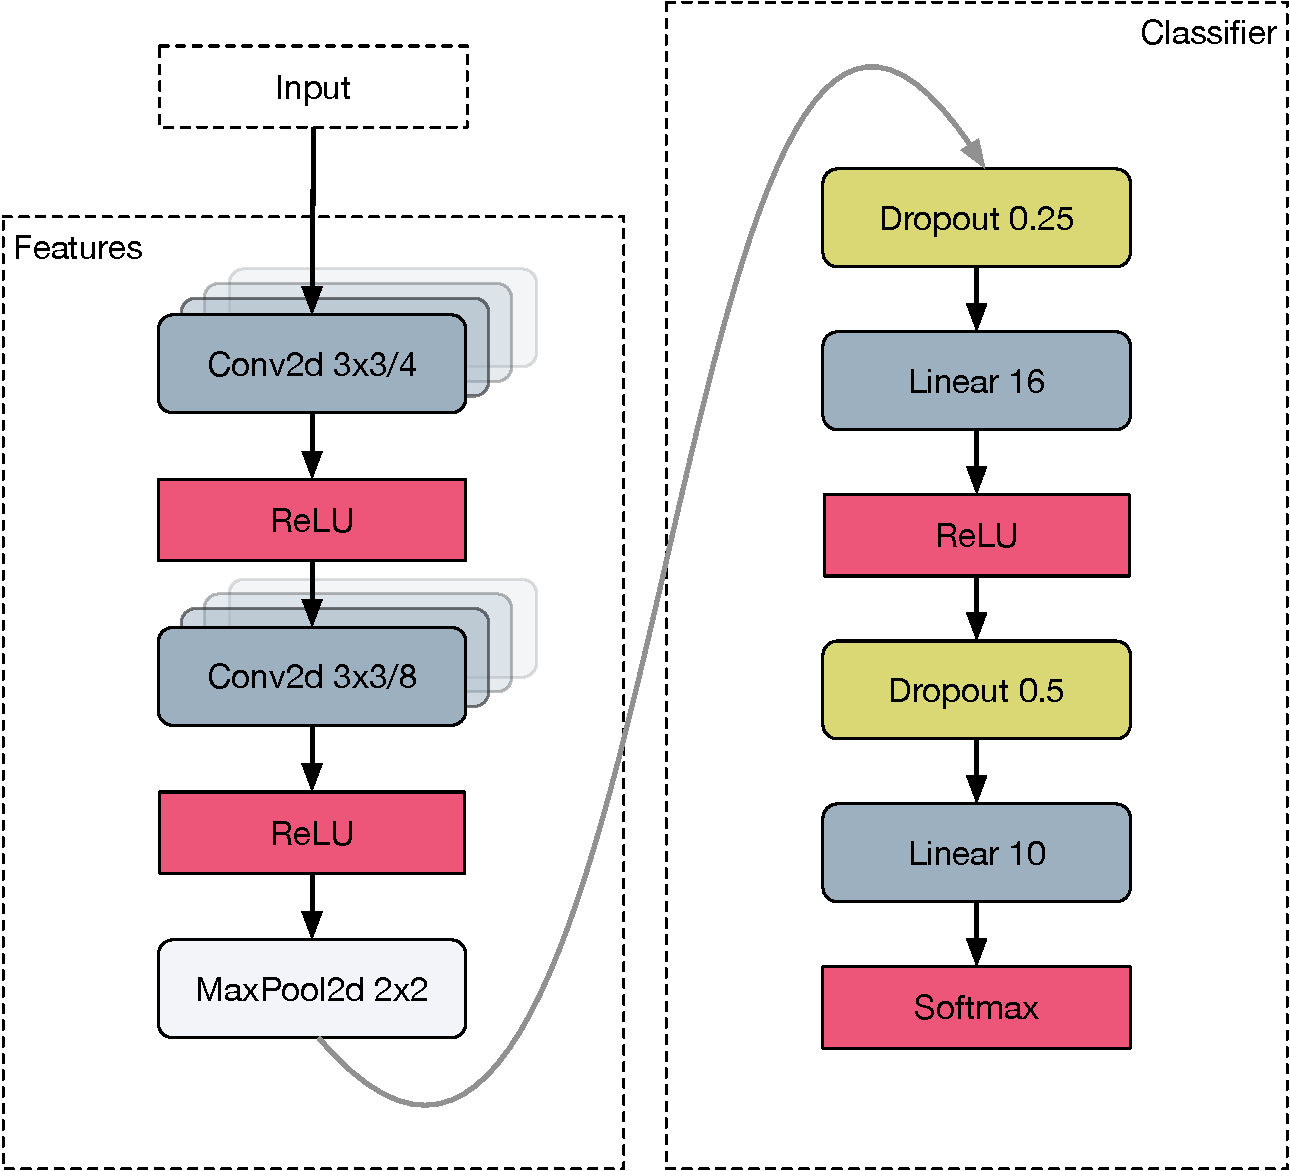
\includegraphics[width=\linewidth]{gfx/diagrams/neural_network/alexnetmini.pdf}
    \caption[Simplified AlexNet architecture]{The network used in this
    experiment. Image features are extracted by $4$ and $8$ convolutional
    filters, respectively, with ReLU nonlinearities. Maximum pooling is applied
    with a filter and stride size of $2$ leading to a resolution a fourth of the
    original size. The classifier portion employs dropout layers to reduce
    co-adaptation of units and a final softmax activation to map outputs to $(0,1)$.}
    \label{fig:alexnetmini}
\end{figure}

In order to validate that there is room for improvement (i.e.~the task is not
too easy), the training has been
run about twenty times for both a constant learning rate and an exponentially
decaying rate according to
\begin{equation}
    \eta_{e+1}  = 0.98^{e+1} \eta_{e},
\end{equation}
$e$ being the epoch index.
The final accuracies after $100$ epochs of training for constant learning rate,
exponential decay are shown in \cref{fig:validation1}. As can be seen, there is
a significant improvement when decaying the learning rate over keeping it
constant.

\begin{figure}
    \centering
    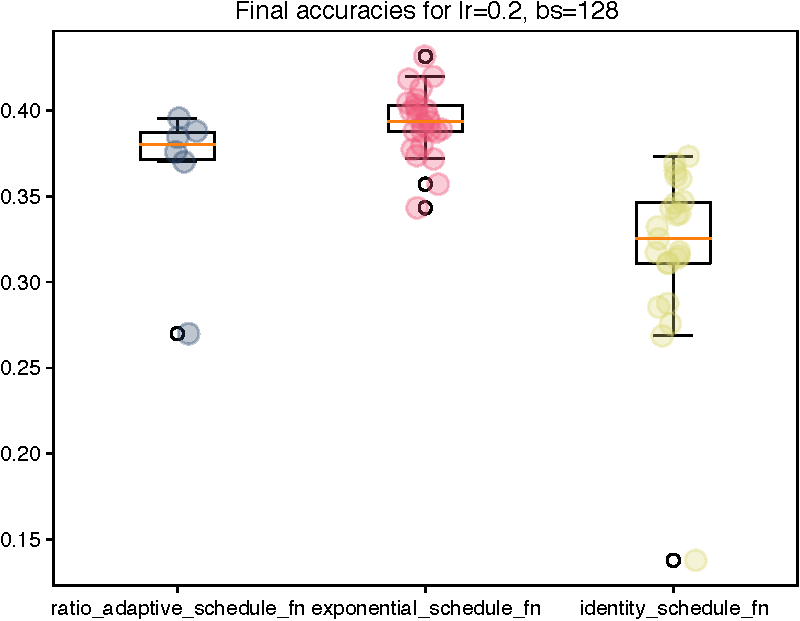
\includegraphics[width=\linewidth]{gfx/diagrams/experiments/experiment_validation.pdf}
    \caption{Final accuracies after 100 epochs}
    \label{fig:validation1}
\end{figure}

As a first proof of concept, an adaptive learning rate based on the ratio
between weight updates and weights is implemented with the help of the library.

Let $l$ be the number of layers with weight matrices associated with them (for
instance linear or convolutional layers, but not activation functions, dropout,
or the like). Let $\left\{W_{i,k} \mid i = 0 \ldots l - 1\right\}$ be the set of weight
matrices at training step $k$.  Let $\eta$ be the base learning rate and
$\frac{1}{t}$ be a target value to which we want the update-to-weigh ratio to
move. Furthermore, let $\gamma \in (0, 1)$ be a decay factor for exponential
smoothing.  Now, let

\begin{equation}
    R_{i,k} = \frac{||W_{i,k} - W_{i,k-1}||_2}{||W_{i,k}||_2}
\end{equation}

be the ratio between the $L2$-Norms of layer $i$'s weight updates before step $k$ step
and the weights at step $k$ themselves.  We then select the new learning rate
for batch step $k+1$ as

\begin{align}
    \eta_{k+1}   = \eta_{k}
                   \left(
                   t \cdot \frac{1}{l}
                   \sum_{i=0}^{l-1} \gamma R_k + (1 - \gamma) R_{k-1}
                   \right)^{-1}
\end{align}

for $k \ge 2$.  This is the average exponentially smoothed update-weight-ratio,
divided by the target range. This learning rate is used for vanilla gradient
descent without any other modifications beyond capping it to some value in case
of very small ratios. The effect of adapting the learning rate according to this
schedule is that the average ratio between the weight updates and the weights
moves towards the target range. The idea that the ratio between updates and
weights is a quantity which should be constrained has not been extensively
investigated. The claim is made by \citet{karpathycs231n}, who states that a
target of $\frac{1}{t} = 10^{-3}$ is a reasonable value.
\cref{fig:schedule-accuracies} displays a set of accuracy traces for each of the
schedules (constant, exponential decay, ratio-adaptive) with different base
learning rates. The network was trained from scratch $5$ times for each combination.

The experiment shows surprising results, namely that a this simple scheme of
dynamically adapting the learning rate to the magnitude of weight change at each
training step easily outperforms any constant value for $\eta$ and achieves
almost state-of-the-art accuracy in some cases (the best reported performance
by \citet{shakedrop} is $97.69\%$).

As an impression of how the library presented in \cref{ikkuna} simplifies a
general implementation of such a learning rate schedule, code is provided here.

When an \verb+Exporter\+ is configured for a given model, a
\verb+RatioSubscriber+ (see \cref{tbl:subscribers}) must be added to the message
bus in order for the update-weigh-ratio ($R_{i,k}$ in the above equations) to be
published. One can then subscribe them and process the information with this
subscriber:
\begin{lstlisting}[language=Python]
class RatioLRSubscriber(PlotSubscriber):
    def __init__(self, base_lr, smoothing=0.9, target=1e-3, max_factor=500):
        subscription = Subscription(self, ['weight_updates_weights_ratio', 'batch_started'],
                                    tag=None, subsample=1)
        super().__init__([subscription], get_default_bus(),
                         {'title': 'learning_rate',
                          'ylabel': 'Adjusted learning rate',
                          'ylims': None,
                          'xlabel': 'Train step'})
        # exponential moving avg of R_{i,k}
        self._ratios     = defaultdict(float)
        # maximum multiplier for base learning rate (in pathological cases)
        self._max_factor = max_factor
        # exp smoothing factor
        self._smoothing  = smoothing
        # target ratio
        self._target     = target
        # this factor is always returned to the learning rate scheduler
        self._factor     = 1
        self._base_lr    = base_lr

    def _compute_lr_multiplier(self):
        '''Compute learning rate multiplicative. Will output 1 for the first batch since no layer
        ratios have been recorded yet. Will also output 1 if the average ratio is close to 0.
        Will clip the factor to some max limit'''
        n_layers = len(self._ratios)
        if n_layers == 0:   # before first batch
            return 1
        else:
            mean_ratio = sum(ratio for ratio in self._ratios.values()) / n_layers
            if mean_ratio <= 1e-9:
                return 1
            else:
                factor = self._target / mean_ratio
                if factor > self._max_factor:
                    return self._max_factor
                else:
                    return factor

    # invoked by the runtime for each incoming message
    def compute(self, message):
        if message.kind == 'weight_updates_weights_ratio':
            # the `key` property for these messages will be the module/layer
            # here we compute the exponential moving average of ratios
            i               = message.key
            R_ik            = message.data
            R_ik_1          = self._ratios[i]
            gamma           = self._smoothing
            self._ratios[i] = (gamma * R_ik + (1 - gamma) * R_ik_1)
        elif message-kind == 'batch_started':
            # before a batch starts, update the lr multiplier
            self._factor = self._compute_lr_multiplier()

    def __call__(self, epoch):
        return self._factor
\end{lstlisting}

The subscriber implements the \verb+__call__()+ method so it can be dropped into
PyTorch's learning rate scheduler (\verb+torch.optim.lr_scheduler.LambdaLR+).
This learning rate schedule can thus be used in every model, without modification.
